\documentclass[10pt, conference, compsocconf]{IEEEtran}

\usepackage{capt-of}
\usepackage{graphicx}
\usepackage{subfig}
\usepackage{booktabs}
\usepackage{multirow}
\usepackage{siunitx}
\usepackage{multicol}
\usepackage{array}
\usepackage{amsmath}
\newcommand{\nltable}[2][c]{%
  \begin{tabular}[#1]{@{}c@{}}#2\end{tabular}}
\newcommand{\wave}{\raise.17ex\hbox{$\scriptstyle\mathtt{\sim}$}}

\newcolumntype{C}[1]{>{\centering\let\newline\\\arraybackslash}m{#1}}

\begin{document}
\bstctlcite{IEEEexample:BSTcontrol}

\title{Approach of Matrix Multiplication on Cloud Distributed System}


\author{\IEEEauthorblockN{Myungjun Son}
\IEEEauthorblockA{Department of Computer Science\\
Kookmin University\\
Seoul, South Korea\\
smj8612@kookmin.ac.kr}
\and
\IEEEauthorblockN{Kyungyong Lee}
\IEEEauthorblockA{Department of Computer Science\\
Kookmin University\\
Seoul, South Korea\\
leeky@kookmin.ac.kr}
}

% make the title area
\maketitle

\begin{abstract}
Abstract
\end{abstract}

\IEEEpeerreviewmaketitle

\section{Introduction}\label{sec:intro}
Big data analytics systems are deployed in cloud computing environments to process ever-increasing dataset while guaranteeing stable operations; scalability and fault-tolerance from the perspective of infrastructure. To satisfy application demands from distinct use cases, cloud computing service providers offer various types of instances that applications can run. Using those resources, most big data platforms are deployed in a scale-out manner. As managing distributed datasets and tasks running on large-scale machines are challenging, abstractions of distributed datasets and resources are crucial to let application developers focus on tasks that really matter. Many systems are proposed to provide a simple and easy interface to handle large-scale datasets, to name a few, Hadoop~\cite{hadoop}, Spark~\cite{spark}, and recently TensorFlow~\cite{tensorflow}.

In analyzing massive dataset to extract valuable insights, matrix multiplication is widely used. In recommendation systems, for example, matrix factorization algorithms, such as SVD, NMF~\cite{nmf}, whose core computation kernel is matrix-matrix multiplication are commonly used. The matrix-vector multiplication is the core kernel in page-rank algorithmby using Power method to get principle eigen vectors~\cite{pagerank}.


%The importance of matrix multiplication
% mention the figure
% briefly mention other approaches to cover cloud configuration recommendation
% summarize proposed method
% summarize the result
% itemize the contributions
\begin{figure}[!ht]
  \centering
  \subfloat[Performance of different instance types of 2xlarge]{\label{fig:different-instance-types}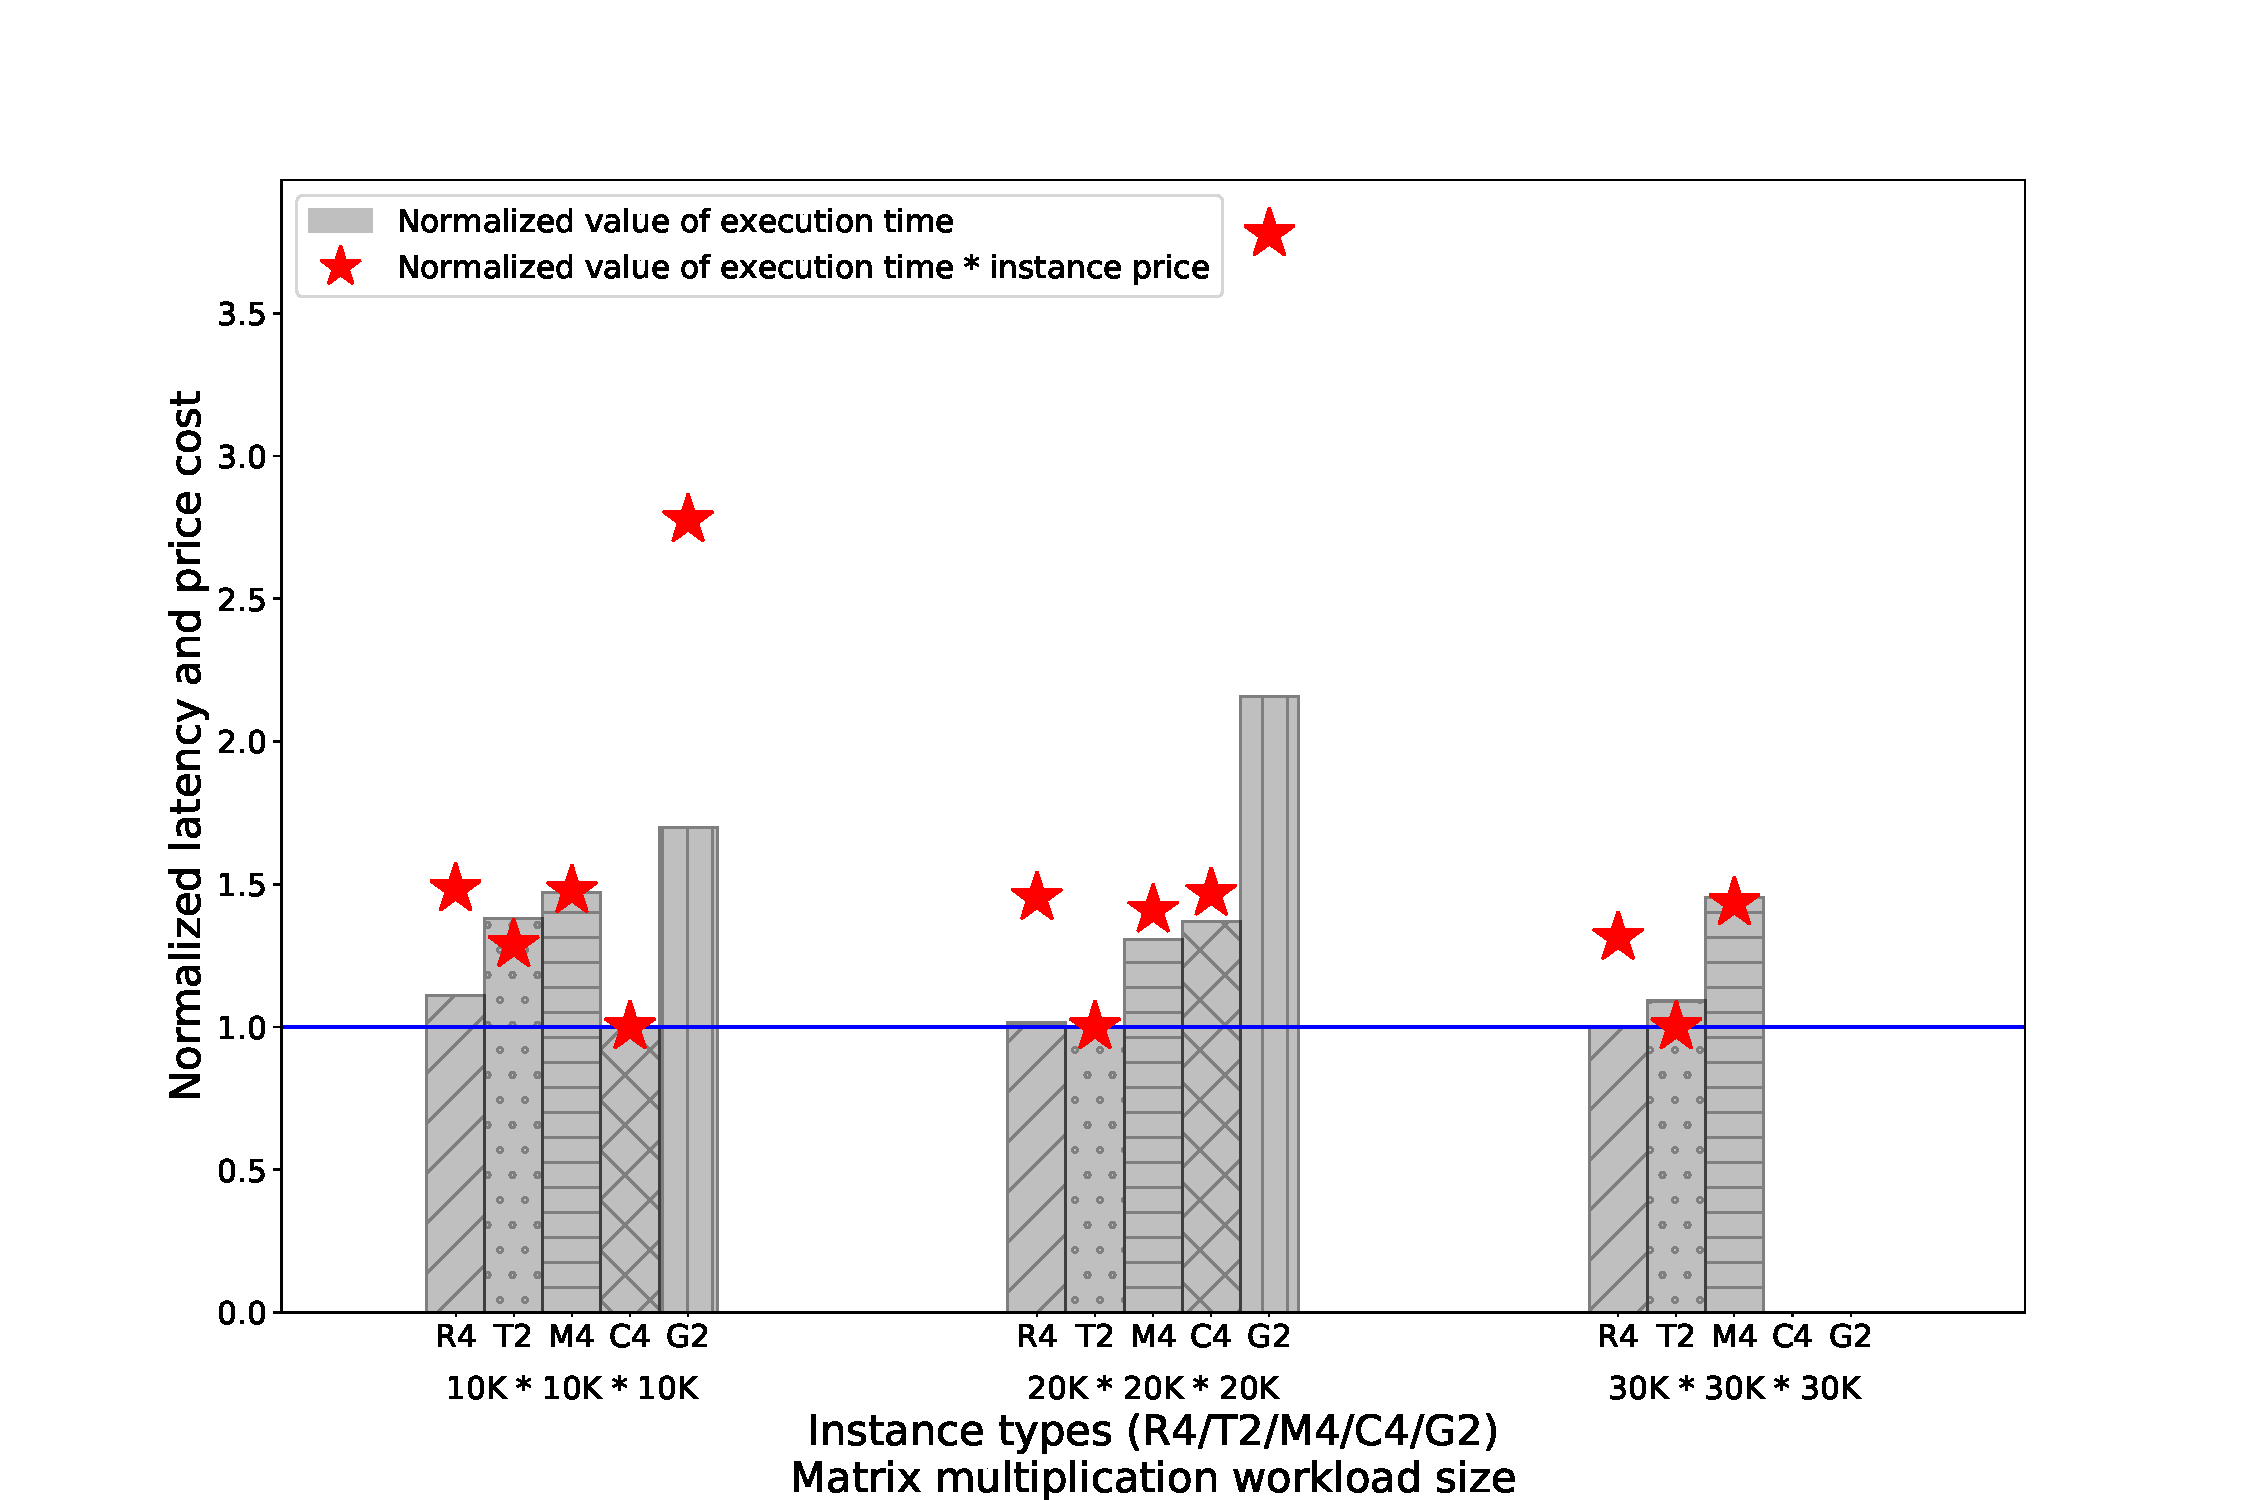
\includegraphics[width=0.5\textwidth]{figures/instance-2xl-compare.pdf}}\\
  \subfloat[Performance of different matrix shapes]{\label{fig:different-matrix-shapes}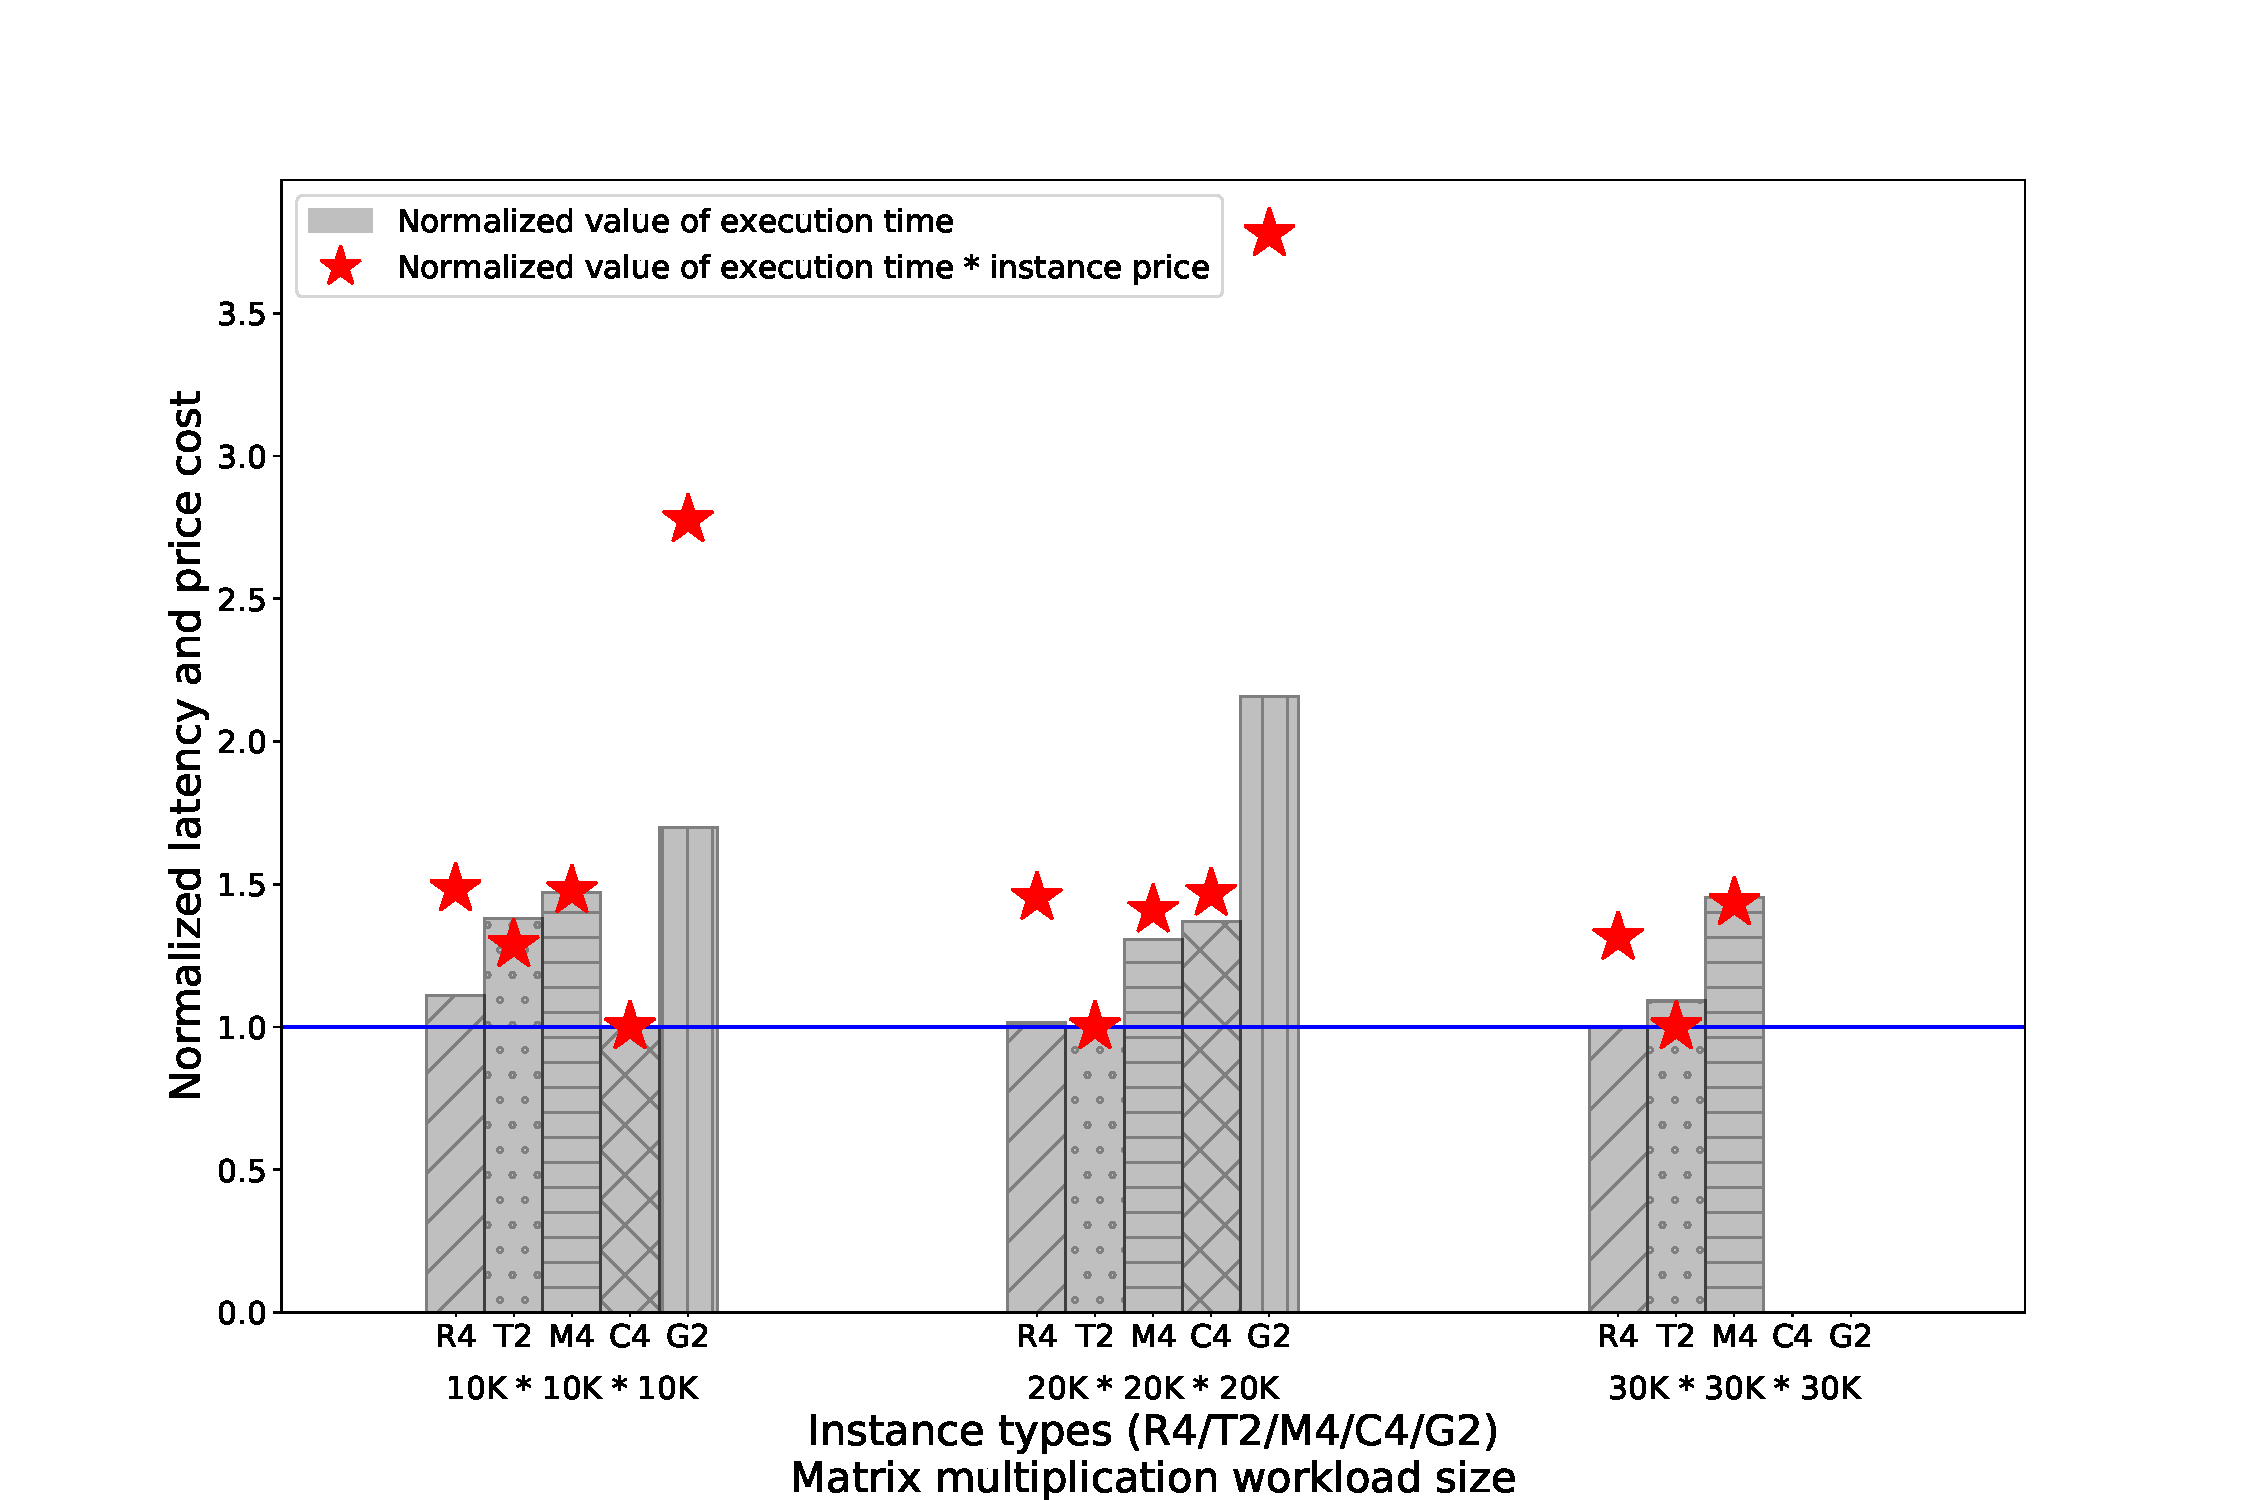
\includegraphics[width=0.5\textwidth]{figures/instance-2xl-compare.pdf}}
  \caption{\label{fig:instance-blocks-sizes-compare}. The normalized value of latency with respect to different instance types and input matrix shapes - the lower, the better.}
\end{figure}

\section{Matrix Multiplication on a Distributed Computing Environment}\label{sec:distributed-matrix-computation}
% explain how the matrix computation happens in spark - mention the step of shuffle, compute, reduce
% How block matrix multiplication happens with the overhead (shuffle, compute, reduce)

Apache Spark is a popular open-source platform for large-scale data. The primary abstraction in Spark is that of a Resilient Distributed Dataset(RDD), which represents a read-only collection of objects partitioned across a set of machines. Spark manages data using partitions that helps parallelize distributed data processing with minimal network traffic for sending data between executors~\cite{spark}. 

As described in Figure~\ref{fig:matmul-whole}, the workflow of matrix multiplication can be mainly divided into three steps in terms of latency occurrence. In \textit{shuffle} step, the output of previous \textit{shuffle} step is transferred through the \textbf{network} in order to get related blocks together for the next step.

In \textit{compute} step, two related submatrices execute cross product locally using the native linear algebra library, OpenBLAS. this step is dependent on \textbf{clock rate}. After three steps, the last step is \textit{reduce} step gathering related cross product and summing these partial results together through \textbf{network}.

\subsection{Matrix Multiplication Overhead Modeling}
For a task of multiplication of two arbitrary size matrices, we analyze the overhead with a different number of available resources for the computation and unique formation of input matrices. For input left ($M_L$) and right ($M_R$) matrices, let us assume the number of rows of the left matrix is $r$, the number of columns of the right matrix as $c$. The number of columns of a left matrix and the number of rows of the right matrix is $k$. We denote the number of worker machines in a cluster as $n$.

On a distributed big data analytics engine, the degree of task parallelism is mainly dependent on the number of input matrix partitions and workers. In Apache Spark, the parallel execution of matrix multiplication task is achieved by dividing the output matrix to multiple blocks and computing each output block independently after fetching corresponding chunks from the left and right input matricies~\cite{spark-mm}. Deciding the optimal partitioning scheme of left, right, and output matrices with any number of resources are one of our on-going work. In this work, we focus on cases where the number of worker nodes is the squares of the arbitrary integer value, such as 1, 4, 9, etc. With this assumption, the input and output matrices are partitioned in a way that achieves the best parallelism, and this partitioning scheme is officially supported in the reference Spark matrix multiplication method~\cite{spark-mm-code}.

\subsection{Overhead Modeling with Different Number of Resources}\label{sec:overhead-number-of-nodes}
With $n$ worker nodes, where $n$ is a squared number of any arbitray number, to achieve the best parallelism, input and output matricies are block-partitioned (Section \ref{fig:blockmatrix}) that the dimension of left, right, and output blocks is $\sqrt{n} \times \sqrt{n}$. The number of elements in each block of the left matrix is $\frac{r \times k}{n}$, right matrix is $\frac{k \times c}{n}$, and the output matrix is $\frac{r \times c}{n}$.

With the above block-partitioned scheme, in the fetch and shuffle step, as we increase the number worker nodes, $n$, each block in the left and right matrices are required to be fetched and shuffled $\sqrt{n}$ times; the number of row/column blocks in the output matrix. As the size of each block is proportional to $\frac{1}{n}$, per worker fetch and shuffle overheads scale proportional to $\frac{1}{\sqrt{n}}$. With respect to the compute overhead, each output block that is assigned to a worker node needs to compute $\frac{r}{\sqrt{n}}\times k \times \frac{m}{\sqrt{n}}$. Thus, the compute overhead scales proportional to $\frac{1}{n}$.

In summary, in multiplying two matrices, increasing the number of worker nodes decreases the per-node fetch and shuffle overhead with the ratio of $\frac{1}{\sqrt{n}}$. The compute overhead decreases with the ratio of $\frac{1}{n}$. Note that the instance usage cost increases with the ratio of $n$.

% Mention how different formation (square, long-thin, wide-fat) have impact on each overhead

\section{Evaluation}{\label{eval}}

\section{Related Work}\label{sec:relatedwork}
\textbf{Instance Recommendation:} Ernest~\cite{venkataraman2016ernest} predicts performance for different VM and cluster sizes, targeting machine learning analytics applications. PARIS~\cite{Yadwadkar:2017:SBV:3127479.3131614} takes a hybrid online/offline approach, using a random forest model to predict application performance on various VM configurations based on features such as CPU utilization obtained from profiling. None of these systems consider the I/O overhead modeling in distributed cloud environments with arbitrary matrix shape which can affect matrix computation performance. 

%need taming
\textbf{Analyzing performance of data analytics frameworks:} While previous studies have analyzed how CPU, memory, network and storage resources affect Spark performance ~\cite{196352,li2014tachyon,ousterhout2015making} our work is the first to take consideration that I/O overhead can affect shape of the matrix. 

% need taming
% cloud computing performance prediction
% instance recommendation (Ernest, Paris, CCGrid 2017)
% Matrix multiplication performance and Spark + Matrix multiplication

\section{Conclusion and Future Work}
Conclusion~\cite{tr-spark}


\bibliographystyle{IEEEtranS}
\bibliography{abc2}
\end{document}
